\chapter{Applications}
\section{Power-law noise}

We applied the statistical test mentioned in the previous chapter on computer-generated power-law noise series.

A collection of independent and identically distributed observations from a continuous random variable is usually referred to as ``white noise.''
Its power spectrum is constant.
Other types of noise can be obtained stipulating different shapes of the power spectrum.
One of the most common ways to achieve this is by imposing spectra of the form $1/f^k$, where $f$ if the frequency and $k$ is a constant.
The case $k=0$ reverts to white noise;
if $k=1$ one has pink noise;
if $k=2$ one has Brownian noise, also called ``red noise;''
if $k=10\log_{10}2\approx 3.01$ per octave one has blue noise;
if $k=20\log_{10}2\approx 6.02$ per octave one has violet noise.
The Wikipedia page ``Colors of Noise'' available at \url{https://en.wikipedia.org/wiki/Colors_of_noise} discusses other types of noise, where they are used, and how they are called.
Timmer and König~\cite{Timmer1995} discussed ways of simulating $1/f^k$ noise.

Our study forms $k$ by choosing
$k_1\in\{1,3,5\}$, and for each $k_1$ value, we defined $k$ as $k=(k_1-e^0,k_1-e^{-1},k_1-e^{-2},k_1-e^{-3},k_1,k_1+e^{-1},k_1+e^{-2},k_1+e^{-3})$. 
The statistical test is used on every possible pair of a value from $k_1$ and each of its generated $k$ values, using series of \num{1000} observations. 
The hypothesis is rejected if the $p$-value is less than $0.05$, and we iterated ten times for each pair. 

Fig.~\ref{fig:PowerLawTests} shows the rejection rate for each $k_1$. 
The last plot shows the proportion of NaNs produced by the tests.
Power-law series with $k=5$ have entropy around $0.4$, the rest of the time series that will be examined in the paper have entropy above $0.9$, so this should not be a problem. 
The Rejection plot for $k_1=1$ is quite surprising in the sense that many values around $k_1$ have high rejection rate. 
The case $k_1=3$ corroborates that the further away a point gets from $k_1$, the larger is the rejection rate.

\begin{figure}[hbt]
    \centering
    \begin{subfigure}[b]{0.3\textwidth}
        \centering
        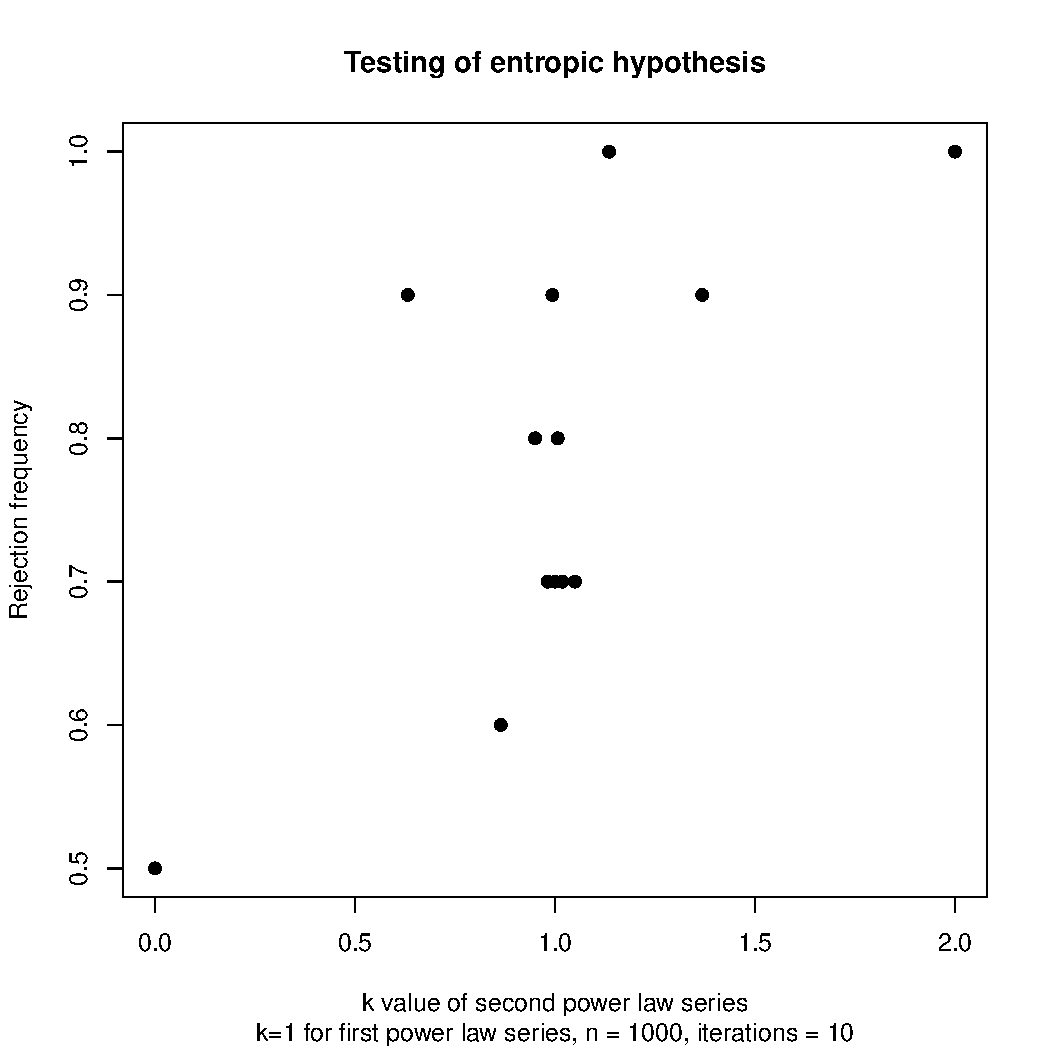
\includegraphics[height=7cm,keepaspectratio]{./powerlaw/rejectionPlot,k1=1,n=1000,iterations=10.pdf}
        % This plot was produced with lines XXX of file YYY; increase the legend size, use serif fonts
    \end{subfigure}
    \hfill
    \begin{subfigure}[b]{0.5\textwidth}
        \centering
        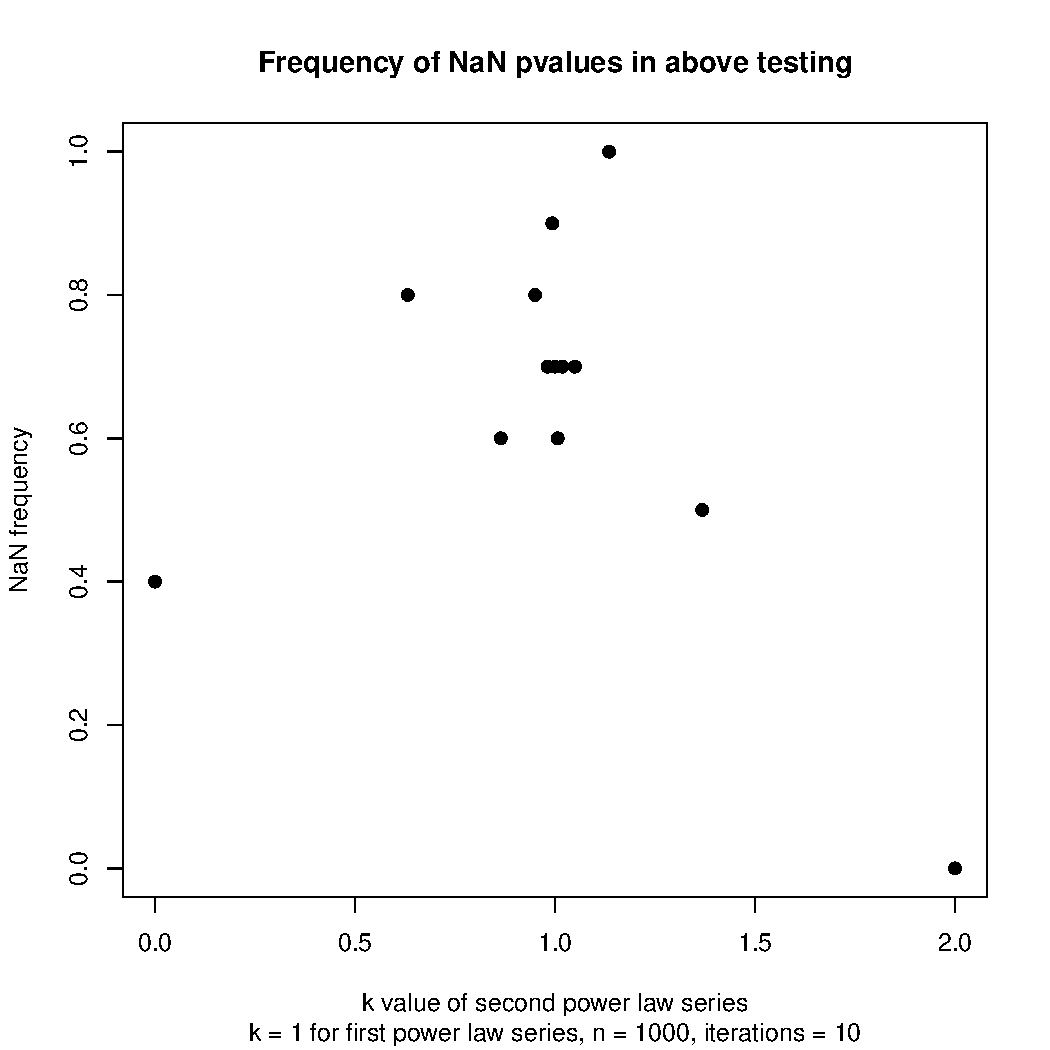
\includegraphics[height=7cm,keepaspectratio]{./powerlaw/NaNPlot,k1=1,n=1000,iterations=10.pdf}
    \end{subfigure}
    \vfill
    \begin{subfigure}[b]{0.3\textwidth}
        \centering
        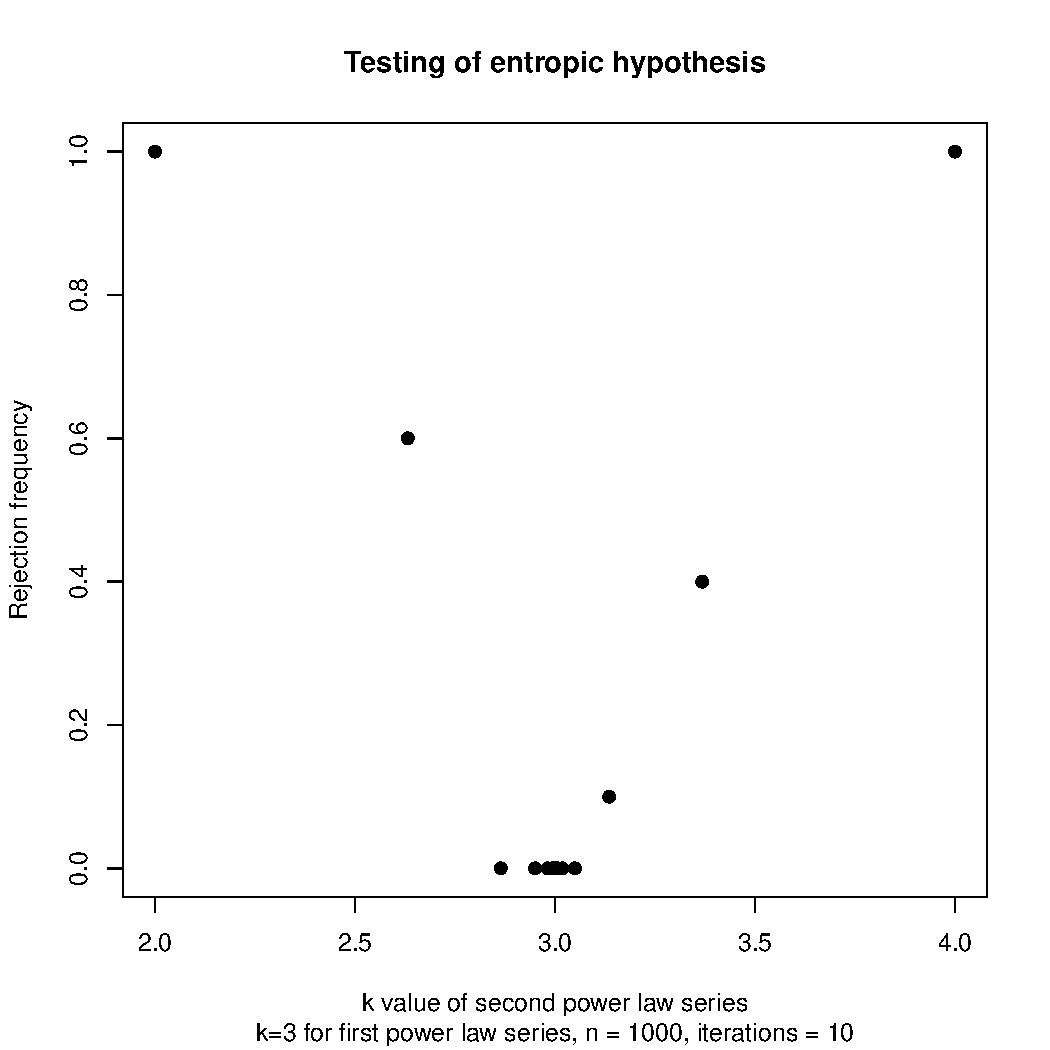
\includegraphics[height=7cm,keepaspectratio]{./powerlaw/rejectionPlot,k1=3,n=1000,iterations=10.pdf}
    \end{subfigure}
    \hfill
    \begin{subfigure}[b]{0.5\textwidth}
        \centering
        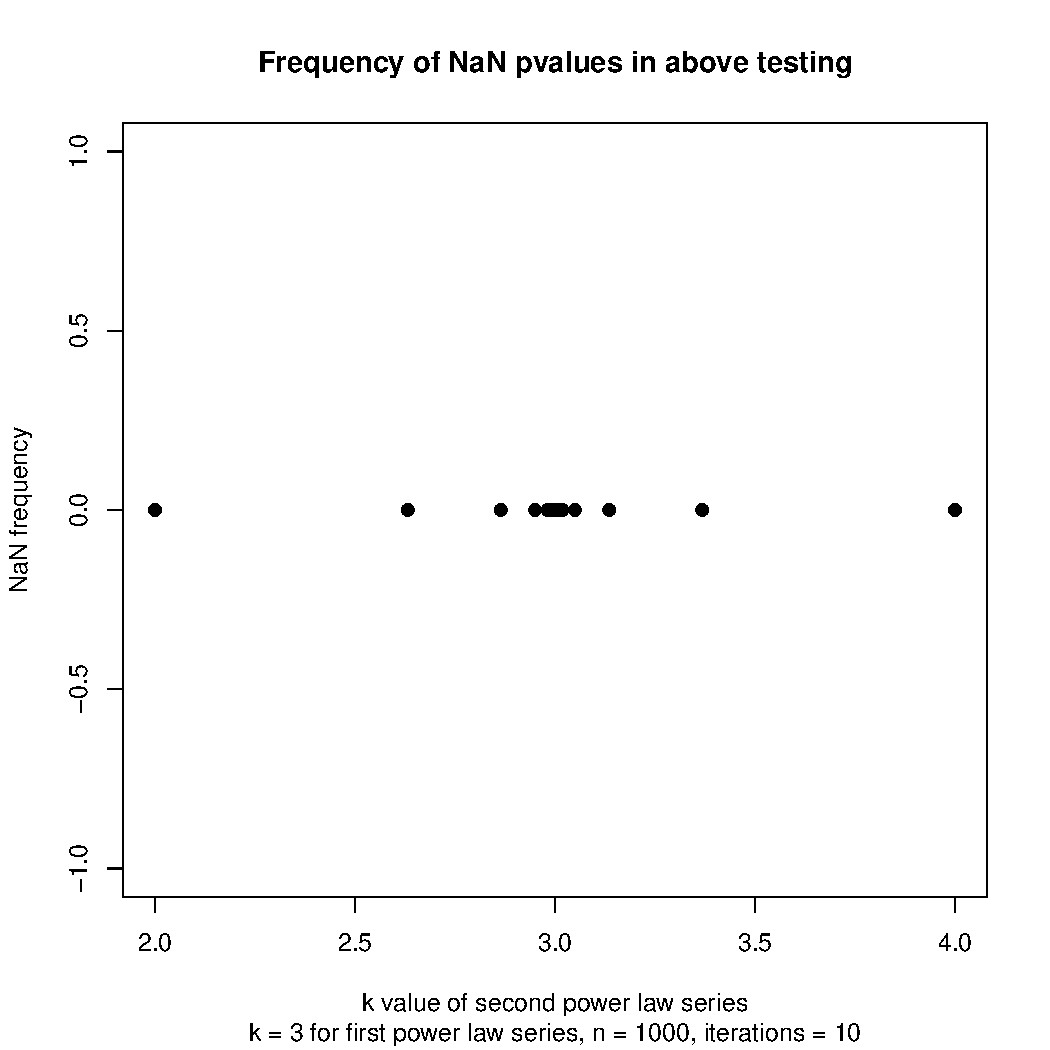
\includegraphics[height=7cm,keepaspectratio]{./powerlaw/NaNPlot,k1=3,n=1000,iterations=10.pdf}
    \end{subfigure}
    \vfill
    \begin{subfigure}[b]{0.3\textwidth}
        \centering
        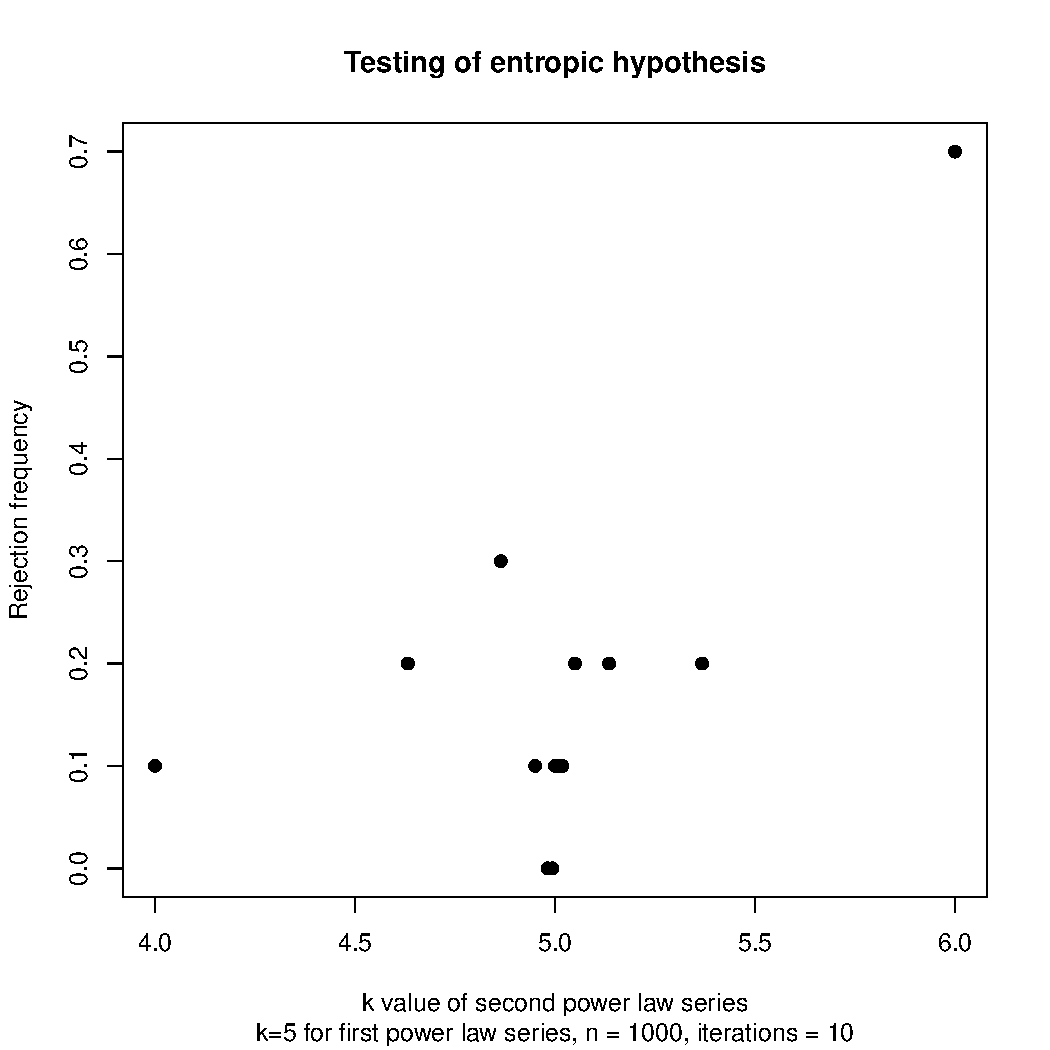
\includegraphics[height=7cm,keepaspectratio]{./powerlaw/rejectionPlot,k1=5,n=1000,iterations=10.pdf}
    \end{subfigure}
    \hfill
    \begin{subfigure}[b]{0.5\textwidth}
        \centering
        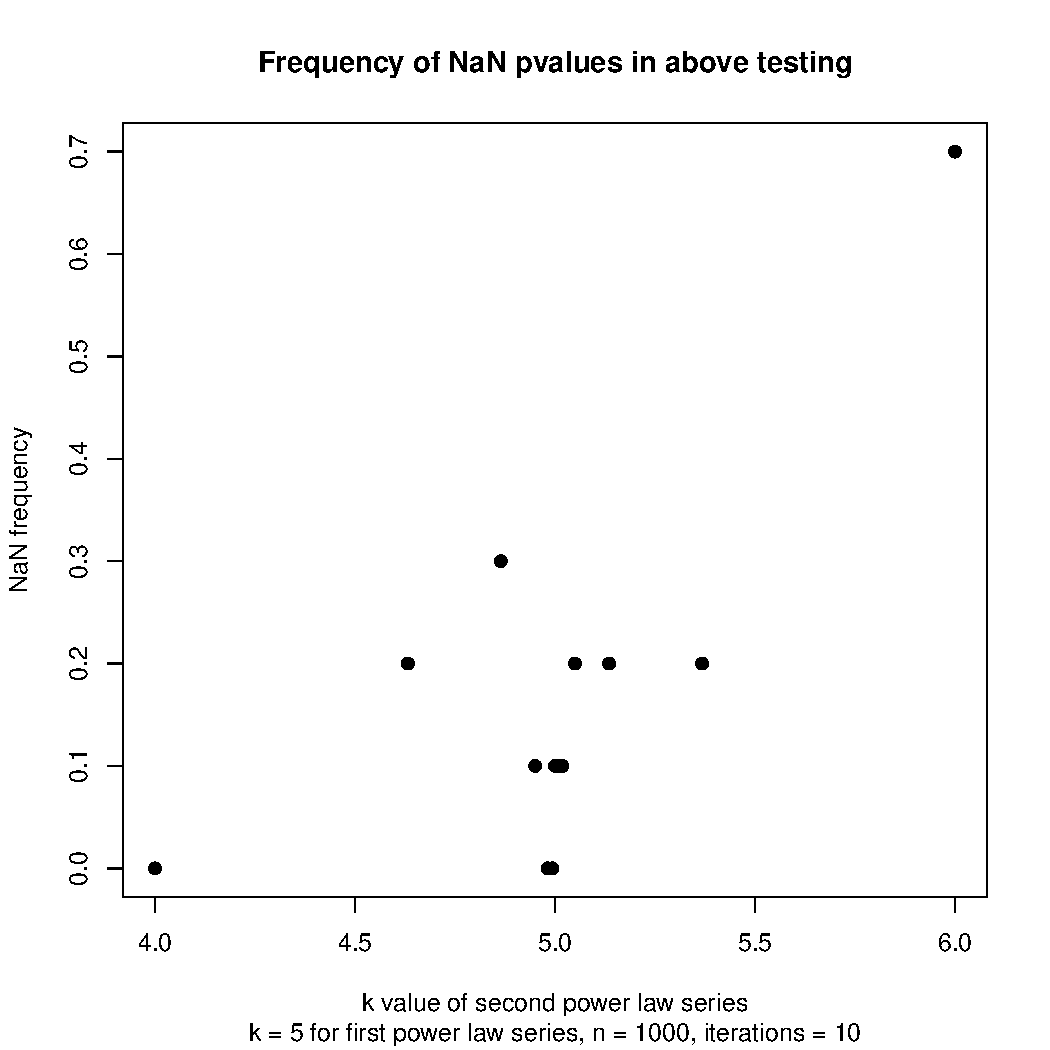
\includegraphics[height=7cm,keepaspectratio]{./powerlaw/NaNPlot,k1=5,n=1000,iterations=10.pdf}
    \end{subfigure}
    \caption{Power-law experiment}\label{fig:PowerLawTests}
\end{figure}

\FloatBarrier

\section{Idea behind new tie breaking}

Ordinal patterns are often used in fields that do science on real-world phenomena. In cases where the measuring equipment finite precision, ties will often occur. 

A person measuring themselves on a scale at different times and weighing the same may not register the same value.
The weight has gone both up and down until a more precise measurement is made, but until that, it is only fair to think both cases are possible and in this case equally possible. 
This type of tie-breaking should work, where it can be argued that a theoretical measurement has a higher precision than the actual measurement. 
It does, however, not make sense to use it when the measured value can be argued to be of the same precision as a theoretical measurement, e.g., “How many cows are in front of me?” 

We will call the proposed solution “Theoretical Split”. 
Note that the theoretical split method does not need to add noise. 
Adding noise almost always removes all ties, which means it should perform identically to the implementation by Chagas et al.~\cite{Chagas2022}, since it is built upon that code. 
The theoretical split and the second tie-breaking solution are deterministic, whereas the Bandt and Pompe solution is stochastic.

As previously mentioned, one of the sources of lack of reproducibility is how tied values are handled.
Bandt and Pompe~\cite{Bandt2002}  in their original paper proposed randomly assigning to the word any of the possible patterns.
Chagas et al.~\cite{Chagas2022} always assigning the same symbol.
Our proposal is to assign an equally large weight to all the possible patterns in case of a tie.

A word of size $D$ should have $D!$ possible patterns.
In the presence of white noise, each of these patterns has weight ${1}/{D!}$. 
The amount of possible patterns is the product of the occurrence of each unique value. 
To calculate the ordinal pattern distribution, simply sum up all the weights for each pattern and divide by the total amount of weight to get the frequency. 

%\FloatBarrier

\section{Temperature Data}

We will partly reproduce the work by Rey et al.~\cite{Rey2023}, with additional plots and tables. 
Only the maximum temperature part of the climate data in section 6 of the article will be used. As can be seen in Table~\ref{tab:TiesPercentages} the percentage of ties in this dataset is extremely high. 
It is therefore quite important to establish how ties are handled since they make up a bulk of the dataset. 

\begin{table}[hbt]
\centering
\begin{tabular}{*5{c}}
\toprule
Location & $D=3$ & $D=4$ & $D=5$ & $D=6$\\ \midrule
Miami & 41.9 & 61.6 & 75.9 & 85.5\\
Edinburgh & 27.2 & 45.1 & 61.4 & 74.5 \\
Dublin & 26.5 & 44.5 & 61.1 & 74.8\\ \bottomrule
\end{tabular}
    \caption{Percentage of ties}\label{tab:TiesPercentages}
\end{table}

%%% ACF Up to this point on 2024-06-03 16:46
The libraries mentioned earlier all handle ties differently, as seen in Figure 4.3. The first three columns are the setting of each experiment. The start date column is included, because the paper, where the data is from, accidentally started their data on 1992-08-14, instead of 1992-08-08 as they said the data started from, it does however not make a big difference, which can be seen between the top three rows and bottom three rows.  If all the values in a row are identically, that means the libraries perform identically. The only setting, where this happens, is when noise is added and Na values are omitted. Na omit removes Na values and the dataset is pushed together, where the Na values have been removed. In the rest of the experiment, this setting will be used. 

\begin{figure}
    \centering
    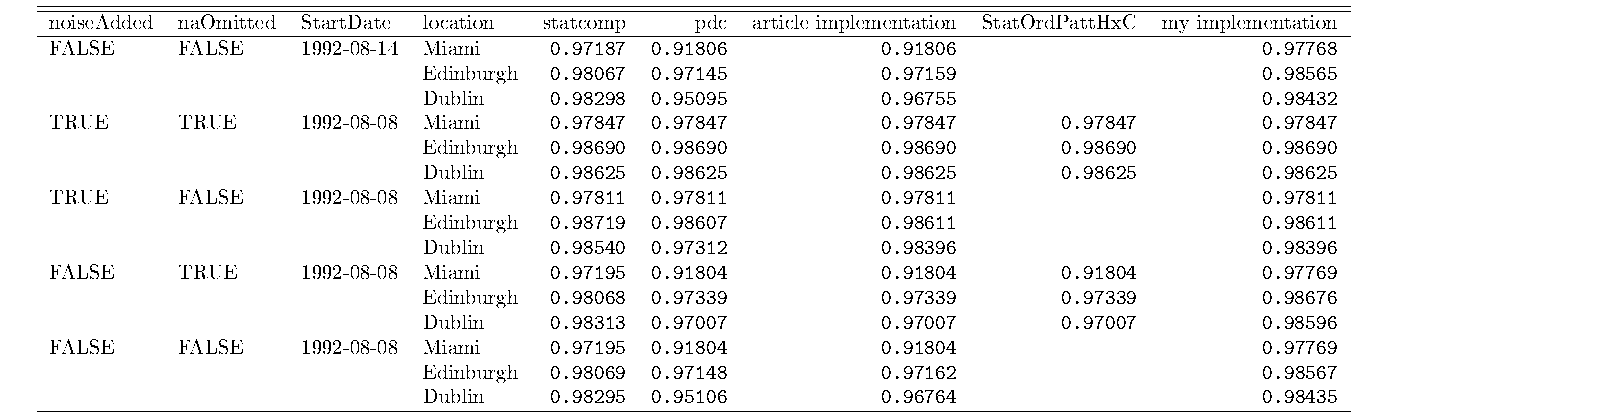
\includegraphics[width=\textwidth,keepaspectratio]{./Weather/entropyTable.pdf}
    \caption{Entropy table of libraries performs on different preprocessing}
\end{figure}

A more in-depth analysis of the Theoretical Split versus adding noise is made. The statcomp library is the comparison library, but it does not matter, which library is chosen, since they perform identically in this case. As can be seen in Figure 4.5 the theoretical value is very close to both the mean and median of the entropy of 1,000 iterations. Figure 4.4 clearly shows the problem of adding a random sample of white noise, since the values are distributed in an interval of range size around 0.003-0.004. The theoretical value is very precise, when comparing both with the median and mean of the 1,000 iterations of noise.

\begin{figure}
    \centering
    
\includegraphics[width=\textwidth,keepaspectratio]{./Weather/noiseStochasticTheoretical.pdf}
    \caption{Iterations of adding noise vs theoretical split in sorted order, the vertical line is median and horizontal is theoretical split value.}
\end{figure}

\begin{figure}
    \centering
    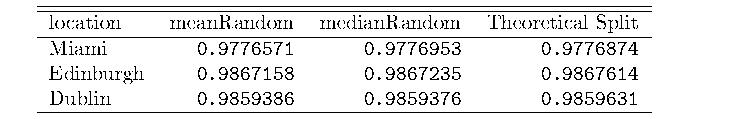
\includegraphics[width=\textwidth,keepaspectratio]{./Weather/random_vs_theoreticalSplit.pdf}
    \caption{Table of mean and median of adding noise and theoretical split. Temperature dataset}
\end{figure}

The above experiment is repeated, but where the theoretical split is fed a constant dataset. The constant values here represent very imprecise measurements, where the true values of the observed phenomenon are assumed to be different. E.g. trying to measure white noise, with a bad instrument. It is important to note that if a dataset contains just a single constant value, where the measurement is precise. The entropy would naturally be 0, since there is full predictability, e.g. “how many cows are on the field at a given time”. The iterations are calculated on random numbers, which ideally should be white noise. Figure 4.6 rarely has the entropy of ideal white noise, which is 1, where the theoretical split can correctly calculate that the poorly measured white noise has entropy 1. Figure 4.7 shows that the median measurement is closer than the mean to the theoretical split, so it might be a better measurement. In Figure 4.5 the median is generally also closer to the theoretical split. 

\begin{figure}
    \centering
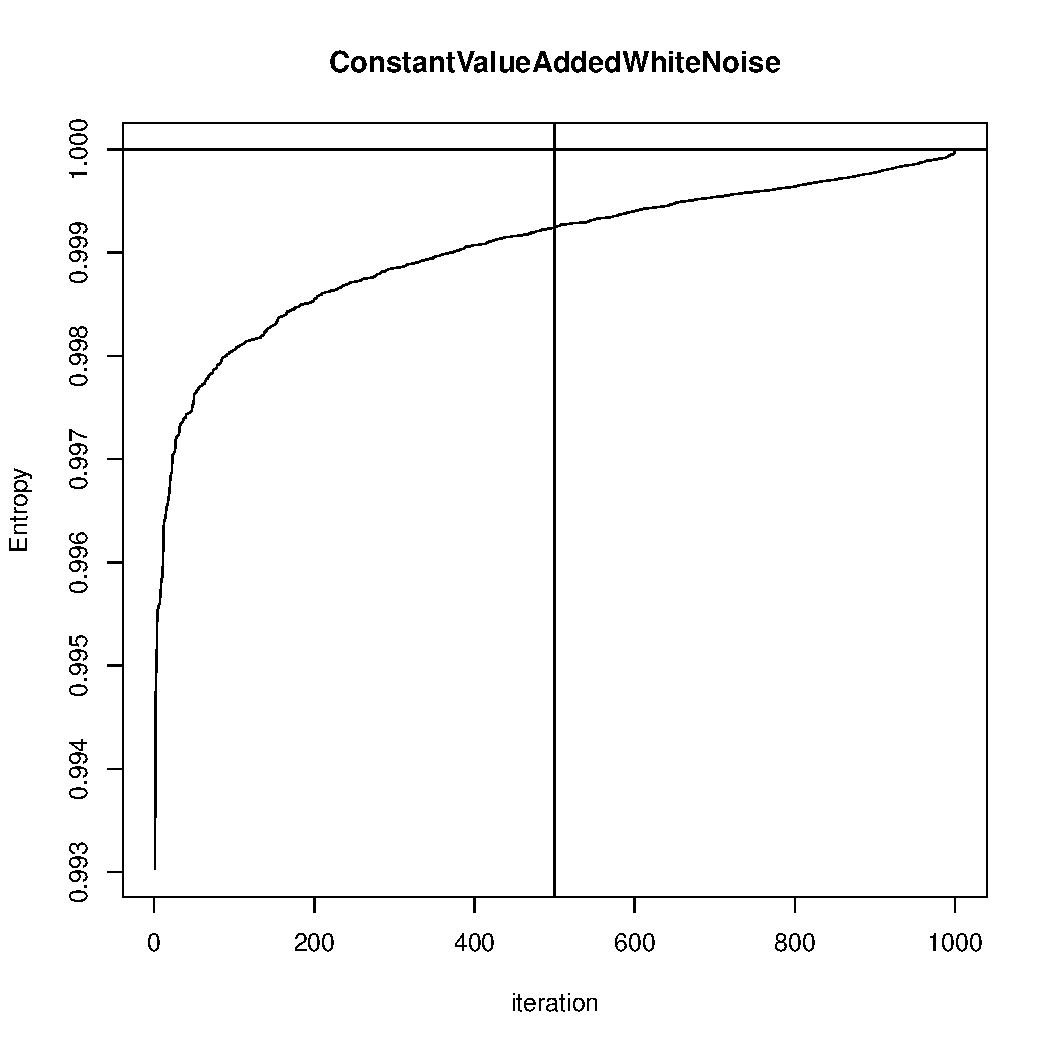
\includegraphics[width=\textwidth,keepaspectratio]{./Weather/constantWithWhiteNoiseStochasticTheoretical.pdf}
    \caption{Constant dataset}
\end{figure}

\begin{figure}
    \centering
    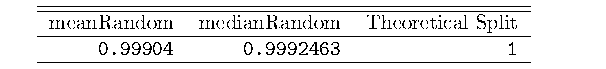
\includegraphics[width=\textwidth,keepaspectratio]{./Weather/random_vs_theoreticalSplitWhiteNoise.pdf}
    \caption{Mean and median of adding noise and theoretical split, constant dataset.}
\end{figure}

Figure 4.8 is a plot of the theoretical split values as the entropy of the three locations on the HxC plane, with confidence intervals on the entropy. At first glance, it looks like the confidence interval sticks out of the boundaries, however it is important to remember that a change in entropy leads to a change in complexity, so the confidence intervals are not breaking the boundaries, since it is impossible for a point to be outside the boundaries.

\begin{figure}
    \centering
    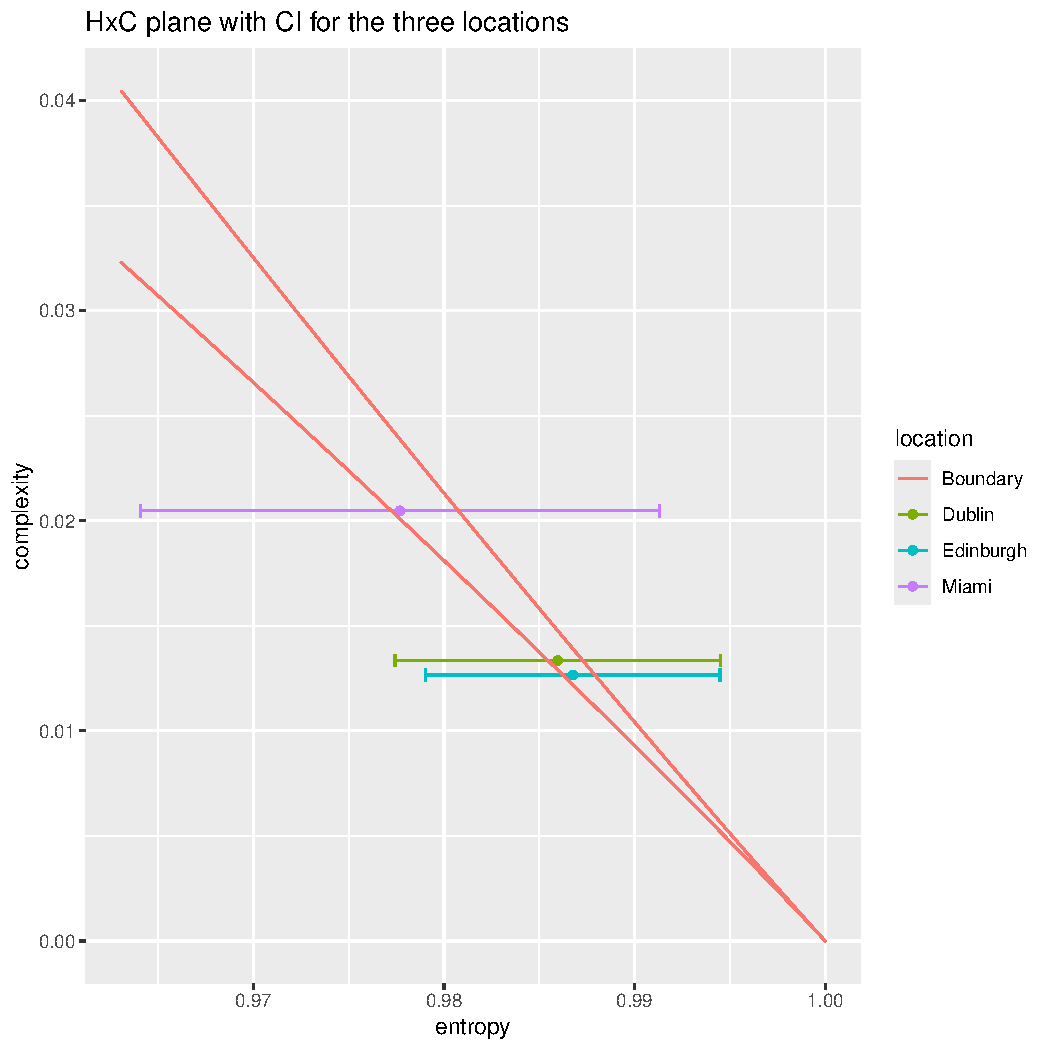
\includegraphics[width=\textwidth,keepaspectratio]{./Weather/confidenceIntervalPlot.pdf}
    \caption{HxC plane of locations with confidence interval}
\end{figure}

P values are calculated. 10 iterations are done on adding noise for breaking ties and compared with the p-value of the theoretical split. The theoretical p value is only larger than one iteration for Miami-Edinburgh, two for Miami-Dublin and four for Edinburgh-Dublin, which is OK. Ideally, it should be between iteration 5 and 6. Most importantly, it is the range of the iterations, which definitely confirms it is implemented so what correctly. 


Adding noise has a couple of problems in the sense that it is much more computer-intensive to calculate just 10 iterations compared with the theoretical value once.
'\begin{figure}
    \centering
    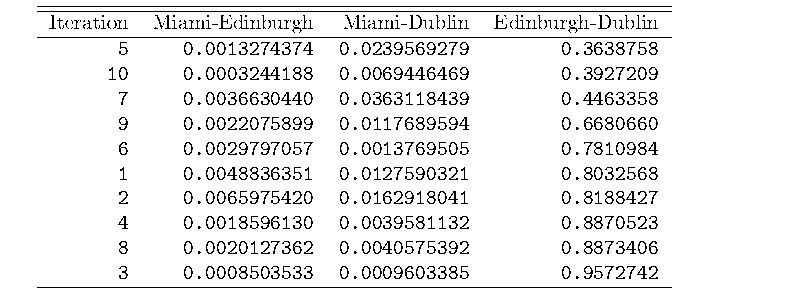
\includegraphics[width=\textwidth,keepaspectratio]{./Weather/pValuesTheoretical,10=Iterations,Sorted.pdf}
    \caption{Noise added, 10 iterations, sorted by column “Edinburgh-Dublin"}
\end{figure}

'\begin{figure}
    \centering
    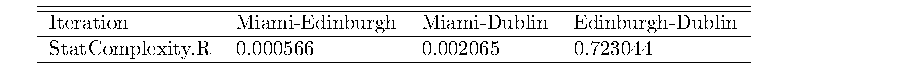
\includegraphics[width=\textwidth,keepaspectratio]{./Weather/pValuesTheoretical.pdf}
    \caption{p value, when using theoretical split}
\end{figure}

